%=====================================================================
%  Class 2 — Empirical Application
%  FEA/USP — Climate Course, 2026
%
%  Companion to ../exercise/climate_data_in_R.R. The class IS that script:
%  Part II walks through it section by section, in order, and it is run live.
%
%    Part I   — what has to be decided, and what Brazil offers
%    Part II  — the script, roughly one frame per section
%
%  The \src line on a Part II frame names the script section it came from.
%  Those section numbers are the only link between deck and script, so if you
%  renumber a section in the script, grep this file for "climate\_data\_in\_R".
%
%  Live figures: fig10_two_cities, fig11_two_years, fig12_hot_reference, plus
%  the two screenshots. All three figures are written by the exercise script
%  itself -- run it and they are rebuilt.
%
%  figures/fig01 through fig09 are ORPHANED. They belonged to frames that have
%  since been cut (degree-days, terciles, population weighting, the binning-bias
%  reproduction) and were drawn by scripts that are no longer in this repo.
%  Nothing \includegraphics them. Keep or delete, but do not assume they are
%  reproducible from what is here.
%
%  Build:  pdflatex main.tex && pdflatex main.tex      (twice, for navigation)
%
%  Frames containing code MUST be [fragile]. Placeholders are [[like this]].
%=====================================================================
\documentclass[aspectratio=169,10pt]{beamer}

\usepackage[english]{babel}
\usepackage{climatetheme}

\graphicspath{{figures/}}
\classfooter{Empirical Application}


\title{Climate Course}
\subtitle{Empirical Application}
\author{Nara Morais (FEA/USP)}
\institute{FEA/USP}
\date{2026}

\newcolumntype{L}[1]{>{\raggedright\arraybackslash}p{#1}}

% R code. listings knows R, so keywords, strings and # comments are found for
% us -- no more marking comments up by hand, and % _ # & $ ^ ~ are all literal
% inside a listing, which means URLs and formulas can be pasted in untouched.
%
% listings is not in a bare TinyTeX; install it once with
%   tlmgr install listings
% Frames containing a listing must be [fragile].
\usepackage{listings}

% listings ships an R language, but its keyword list is a dump of base-R
% function names from the 1990s: data, date, file, class, end, start, value,
% mean, max are all in it. On a slide that bolds half the argument names and
% teaches that `date_start` is a reserved word, which it is not. So: our own
% definition, with the keywords R actually reserves and nothing else. Bold then
% means "language keyword", and a function name looks like a function name.
%
% alsoletter is what stops "date_start" being read as `date` + `_start`:
% listings does not count "." or "_" as letters, but R does.
\lstdefinelanguage{Rlang}{
  keywords     = {function, if, else, for, while, repeat, break, next, in,
                  return, TRUE, FALSE, NULL, NA, Inf, NaN, library, require},
  sensitive    = true,
  % "." and "_" are part of an R name; "%" keeps %in% in one piece, which
  % otherwise prints as a literal percent wrapped around a bold `in`.
  alsoletter   = {._\%},
  morecomment  = [l]{\#},
  morestring   = [b]",
  morestring   = [b]',
}

% Rules above and below, no box, no line numbers, no IDE colouring beyond three
% roles. The point of a code slide is that it reads from the back of the room.
\lstdefinestyle{Rstyle}{
  language          = Rlang,
  basicstyle        = \ttfamily\scriptsize\color{climdeep},
  keywordstyle      = \color{climteal}\bfseries,
  commentstyle      = \color{climgrey}\itshape,
  stringstyle       = \color{climorange},
  showstringspaces  = false,
  keepspaces        = true,
  columns           = fullflexible,
  breaklines        = true,
  breakatwhitespace = true,
  breakindent       = 14pt,
  % A long line that had to wrap is marked, so a wrap is never mistaken for a
  % new statement -- the commonest way a code slide misleads people. The marker
  % must be an \mbox and must carry NO colour command: a \color inside postbreak
  % lands in a discretionary list and beamer's colour handling then reads the
  % following \kern as a number ("Missing number, treated as zero").
  postbreak         = \mbox{$\hookrightarrow$\,},
  frame             = tb,
  framerule         = 0.4pt,
  framesep          = 5pt,
  rulecolor         = \color{climgrey},
  aboveskip         = 8pt,
  belowskip         = 6pt,
  xleftmargin       = 0pt,
  % listings makes characters active, which breaks UTF-8 accents on its own.
  % This maps the Portuguese ones back, so "São Paulo" can be typed in a
  % comment exactly as you would type it in RStudio.
  extendedchars     = true,
  literate          =
    {á}{{\'a}}1 {à}{{\`a}}1 {ã}{{\~a}}1 {â}{{\^a}}1
    {é}{{\'e}}1 {ê}{{\^e}}1 {í}{{\'i}}1
    {ó}{{\'o}}1 {ô}{{\^o}}1 {õ}{{\~o}}1
    {ú}{{\'u}}1 {ç}{{\c c}}1
    {Á}{{\'A}}1 {Ã}{{\~A}}1 {É}{{\'E}}1 {Ó}{{\'O}}1 {Ç}{{\c C}}1,
}
\lstset{style=Rstyle}

% \begin{Rcode} ... \end{Rcode}, with per-frame overrides when one slide needs
% smaller type:  \begin{Rcode}[basicstyle=\ttfamily\tiny\color{climdeep}]
\lstnewenvironment{Rcode}[1][]{\lstset{style=Rstyle,#1}}{}

\newcommand{\code}[1]{\texttt{\small #1}}
\newcommand{\cmt}[1]{\textcolor{climgrey}{\textit{#1}}}

% A clickable address that still looks like the rest of the deck: same \code
% mono as every other path on a slide, just live.
%   \wl{bdmep.inmet.gov.br}          -> https:// is prepended
%   \wl[https://doi.org/10.1000/x]{shown text}  -> when the two differ
% Underscores in a displayed name still need escaping (\wl{br\_inmet\_bdmep});
% the URL in the optional argument does not.
\newcommand{\wl}[2][]{%
  \ifx\relax#1\relax
    \href{https://#2}{\code{#2}}%
  \else
    \href{#1}{\code{#2}}%
  \fi}

% A tibble's column-type row: \ty{dbl} prints <dbl> in grey, so a hand-set
% table on a slide reads as the console output it is quoting. Spelled with
% \textless/\textgreater because beamer reads a literal <...> as an overlay
% specification and would swallow it.
\newcommand{\ty}[1]{\textcolor{climgrey}{\textless #1\textgreater}}

% A quoted data frame. Same visual grammar every time one appears: mono,
% booktabs rules, a grey type row under the header, tight columns.
%   \begin{dfbox}{alignment spec} header \\ types \\ \midrule rows \end{dfbox}
\newenvironment{dfbox}[1]
  {\ttfamily\scriptsize\setlength{\tabcolsep}{3.5pt}\begin{tabular}{@{}#1@{}}\toprule}
  {\bottomrule\end{tabular}}

\usetikzlibrary{positioning,calc}

% Progressive reveal INSIDE a tikzpicture. Using \only would change the bounding
% box between overlays and make the whole diagram jump; this draws every element
% on every slide and simply sets opacity 0 until its turn, so nothing moves.
%   \node[visible on=<2->] ... ;
\tikzset{
  invisible/.style={opacity=0},
  visible on/.style={alt={#1{}{invisible}}},
  alt/.code args={<#1>#2#3}{\alt<#1>{\pgfkeysalso{#2}}{\pgfkeysalso{#3}}},
}

% Three levels of text inside a diagram box, so the box has a reading order:
% a mono uppercase eyebrow saying what the box answers, a bold name, and a
% muted sublabel with the detail. Same idea as a figure's title/caption.
\newcommand{\dtag}[2]{{\ttfamily\scriptsize\color{#1}#2}}
\newcommand{\dsub}[1]{{\scriptsize\color{climgrey}#1}}

% One colour per ecosystem, shared by everything inside it. Note this is colour
% used as a *category*, not as emphasis -- so the three are equal in weight and
% none of them is the accent. All three are from the same palette as the theme.
\definecolor{climbrick}{RGB}{155,34,38}

% A group of tools: a filled chip with the ecosystem's name, then a hairline in
% the same hue tying the entries below it together.  \grp{colour}{name}
\newcommand{\grp}[2]{%
  \par\vspace{2pt}%
  \colorbox{#1}{\color{white}\bfseries\scriptsize\strut~#2~}%
  \par\vspace{3pt}{\color{#1!35}\hrule height 0.6pt}\vspace{1pt}}

% One tool inside a group: its name in the group's colour, then what it hands
% you. Same name-then-sublabel ramp as the boxes on frame 2, so a reader who
% learned to read that diagram already knows how to read this slide.
%   \tl{colour}{name}{what it gives you}
\newcommand{\tl}[3]{%
  \par\vspace{4pt}%
  {\ttfamily\bfseries\footnotesize\color{#1}#2}%
  \par\vspace{1pt}%
  {\scriptsize\color{climdeep}#3}\par}

% A screenshot slot: \shot{name}{width}{height}. Draws figures/<name>.png once
% that file exists, and until then a dashed box of exactly the same footprint,
% so the slide can be laid out and checked before the screenshots are taken.
% To fill one in: save the PNG as figures/<name>.png and recompile. No edit here.
\newcommand{\shot}[3]{%
  \IfFileExists{figures/#1.png}%
    {\setlength{\fboxsep}{0pt}\setlength{\fboxrule}{0.4pt}%
     \fcolorbox{climdeep!25}{white}{\includegraphics[width=#2]{figures/#1}}}%
    {\begin{tikzpicture}
       \node[draw=climorange, dashed, line width=0.8pt, rounded corners=3pt,
             fill=climorange!5, minimum width=#2, minimum height=#3,
             align=center, font=\scriptsize, text=climorange]
         {SCREENSHOT\\[2pt]\texttt{figures/#1.png}};
     \end{tikzpicture}}}

%=====================================================================
\begin{document}

\titleframe{Empirical Application}{Brazilian climate data in R}{}


% ---------------------------------------------------------------------
% The sentence first, then the two questions it leaves open, answered in turn:
%   <2>  "climate measures" of WHAT? -> climate data
%   <3>  "visualize" HOW? -> a map, because the differences we care about are
%        geographic
%   <4>  and a map of municipalities needs boundaries -> a shapefile
% Which is also the order the rest of the class runs in: data, then map.
%
% Three drawing rules worth stealing for your own figures:
%   * connectors turn at right angles, never on a diagonal slant;
%   * arrows are muted grey -- an arrow is structure, not emphasis;
%   * the accent colour is spent on exactly two boxes, the two things we
%     actually have to go out and fetch. Accenting everything accents nothing.
\begin{frame}{What we are doing today}
  \vspace{2pt}
  \begin{center}
  \begin{tikzpicture}[
      font=\small,
      w/.style     ={inner sep=1pt, text=climdeep},
      verb/.style  ={inner sep=1pt, text=climteal, font=\small\bfseries},
      obj/.style   ={inner sep=1pt, text=climdeep, font=\small\bfseries},
      card/.style  ={rounded corners=3pt, inner sep=5pt, align=center,
                     text width=3.6cm, text=climdeep, font=\footnotesize},
      plain/.style ={card, fill=white,        draw=climdeep!40,   line width=0.6pt},
      focal/.style ={card, fill=climorange!7, draw=climorange!85, line width=0.7pt},
      aside/.style ={text=climgrey, align=center, text width=3.6cm,
                     font=\scriptsize\itshape},
      ar/.style    ={->, draw=climgrey, line width=0.7pt, rounded corners=3pt}]

    % --- the sentence, one node per word so two of them can carry a branch ---
    \node[w]                      (s1)  {The goal here is to};
    \node[verb, right=2pt of s1]  (s2)  {gather,};
    \node[verb, right=2pt of s2]  (s3)  {analyze};
    \node[w,    right=2pt of s3]  (s4)  {and};
    \node[verb, right=2pt of s4]  (vis) {visualize};
    \node[obj,  right=3pt of vis] (cm)  {climate data};
    \node[w,    right=2pt of cm]  (s7)  {from Brazil.};

    % The midpoint of the sentence, and the line the two boxes sit on. Hanging
    % everything off these two keeps the picture's bounding box centred on the
    % sentence, so \begin{center} puts the whole thing straight rather than
    % centring the branches and dragging the text along behind them.
    \coordinate (mid) at ($(s1.west)!0.5!(s7.east)$);
    \coordinate (row) at ([yshift=-1.2cm]mid);
    % The left column is the right column reflected through the midpoint --
    % (mid)!-1!(cm) is mid minus the vector from mid to cm. Written this way
    % so the two branches stay symmetric if the sentence above is ever reworded.
    \coordinate (mirror) at ($(mid)!-1!(cm|-mid)$);

    % --- right branch: measures OF WHAT? ------------------------------------
    % (cm |- row) is "x from the phrase, y from the row", so this box sits
    % directly under its word and the connector is a plain vertical line. Each
    % connector takes the simplest legal route: straight when the endpoints
    % share an axis, a right-angled elbow when they do not. Never a diagonal.
    \node[focal, visible on=<2->, anchor=north] (data) at (cm |- row)
      {\dtag{climorange!85}{OF WHAT?}\\[2pt]
       \textbf{}\\[1pt]
       \dsub{temperature $\cdot$ precipitation\\ humidity $\cdot$ wind $\cdot$ radiation}};
    \draw[ar, visible on=<2->] (cm.south) -- (data.north);

    % --- left branch: visualize HOW? ----------------------------------------
    \node[plain, visible on=<3->, anchor=north] (map) at (mirror |- row)
      {\dtag{climgrey}{HOW?}\\[2pt]
       \textbf{a map}\\[1pt]
       \dsub{the differences we care about\\ are geographic}};
    \draw[ar, visible on=<3->] (vis.south) -- ++(0,-0.55) -| (map.north);

    \node[focal, visible on=<4->, anchor=north, text width=3.2cm]
      (shp) at ([yshift=-0.7cm]map.south)
      {\dtag{climorange!85}{WHICH NEEDS}\\[2pt]
       \textbf{a shapefile}\\[1pt]
       \dsub{IBGE municipal boundaries}};
    \draw[ar, visible on=<4->] (map.south) -- (shp.north);

    % The forward pointer lands last: everything is on the table, and the very
    % next frame is the four decisions it is pointing at.
    \node[aside, visible on=<4->, anchor=north] at ([yshift=-0.5cm]data.south)
      {Which one, at what resolution, aggregated how? --- next slide.};

  \end{tikzpicture}
  \end{center}
\end{frame}

% ---------------------------------------------------------------------
\begin{frame}{But first, we have to decide four things}

  \begin{enumerate}
    \small
    \item \textbf{Which product?} A station network, an interpolated grid, a
          satellite retrieval, a reanalysis. These are different objects, not
          different accuracies of the same object.
    \item \textbf{How to aggregate space?} Grid cells into municipalities ---
          weighted by what? Area, population, cropland, nothing?
    \item \textbf{Which functional form?} Mean, a count above a threshold,
          degree-days, an anomaly. And: does the averaging happen before or after
          the transformation?
    \item \textbf{Which boundaries?} Municipalities are created and merged. The
          year of the map has to match the year of the aggregation.
  \end{enumerate}
  \src{Dell, Jones \& Olken (2014), \emph{JEL}, Sections 2.3--2.4}
\end{frame}

% =====================================================================
\partframe{Part I}{Where does Brazilian climate data come from?}
% =====================================================================
\section{Part I — Where does Brazilian climate data come from?}

% ---------------------------------------------------------------------
\begin{frame}{The sources}
  \vfill
  \begin{center}
    \small
    \setlength{\tabcolsep}{4pt}
    \renewcommand{\arraystretch}{1.45}
    \begin{tabular}{@{}L{0.19\textwidth}L{0.24\textwidth}L{0.17\textwidth}L{0.33\textwidth}@{}}
      \toprule
      \textbf{Source} & \textbf{What we observe} & \textbf{Example} &
        \textbf{From source to municipality} \\
      \midrule
       Weather stations & Measurement points &
        INMET/BDMEP &
        Assign a station to the municipality, or aggregate the stations \\
      \textcolor{climorange}{\bfseries Grids} & Spatial cells &
        Xavier et al.\ \dsub{(BR-DWGD)} &
        Intersect the grid with the border and aggregate \\
      Satellites & Surface observation pixels &
        MODIS/Landsat &
        Aggregate the pixels inside the border \\
      Reanalyses & Model-based estimates on a grid &
        ERA5 &
        As for grids --- but the values are modelled, not measured \\
      \bottomrule
    \end{tabular}

    \vspace{6pt}
    \dsub{In orange: the source this class uses.}
  \end{center}
  \vfill
\end{frame}

% ---------------------------------------------------------------------
% This used to be four frames, one per source, and all four ended in the same
% arrow. The table above already says what each source is; all this frame owes
% the reader is the catch in each one, and the fact that the last step is
% shared. Four slides of parallel bullets became one slide of four blocks.
\begin{frame}{Same last step, whichever door you come in by}
  \vspace{-2pt}
  \begin{columns}[T]
    \begin{column}{0.48\textwidth}
      {\bfseries\color{climdeep}Weather stations}\\
      \dsub{INMET / BDMEP}\\[2pt]
      {\footnotesize An instrument at a point, reading the air around it. The
       catch is which station stands for a municipality  and most
       municipalities have none.}

      \vspace{10pt}
      {\bfseries\color{climorange}Grids}\ \ \dtag{climorange}{WHAT WE USE}\\
      \dsub{Xavier et al.\ (2022) --- BR-DWGD}\\[2pt]
      {\footnotesize Those same stations interpolated onto a
       $0.1^\circ \times 0.1^\circ$ lattice, daily. Now every municipality has a
       value, including the ones with no thermometer and the catch is
       exactly that: the value is estimated.}
    \end{column}
    \begin{column}{0.48\textwidth}
      {\bfseries\color{climdeep}Satellites}\\
      \dsub{MODIS, Landsat; INPE for Brazil}\\[2pt]
      {\footnotesize Pixels, at fine spatial detail. The catch is the variable:
       MODIS gives \textbf{land surface} temperature . Asphalt at midday is not what a person or a soybean
       experiences.}

      \vspace{10pt}
      {\bfseries\color{climdeep}Reanalyses}\\
      \dsub{ERA5 --- ECMWF / Copernicus}\\[2pt]
      {\footnotesize Observations run through a weather model: hourly,
       everywhere, decades back. The catch is that the values were
       \emph{computed}.}
    \end{column}
  \end{columns}
  \vspace{8pt}
  \begin{center}
    \textbf{stations $\cdot$ cells $\cdot$ pixels} $\rightarrow$
    \textbf{municipality} $\rightarrow$ \textbf{aggregate}\\[3pt]

  \end{center}
  \src{INMET/BDMEP; Xavier et al.\ (2022); MODIS LST (NASA); INPE;
       ERA5 --- ECMWF/Copernicus}
\end{frame}



% ---------------------------------------------------------------------
% The manual route comes first, deliberately. A shortcut only means something
% once you have seen the thing it is a shortcut around -- so: here are the two
% doors at INMET, here is the file that comes out of them, and here is why
% nobody does it this way twice.
\begin{frame}{Getting it yourself}
  \vspace{-4pt}
  \begin{columns}[t]
    \begin{column}{0.48\textwidth}
      \centering
      \shot{shot-bdmep}{0.98\linewidth}{2.7cm}\\[4pt]
      {\footnotesize\textbf{BDMEP} --- \wl{bdmep.inmet.gov.br}}\\[1pt]
      {\scriptsize\color{climgrey}Choose stations, dates, variables. Get one CSV.}
    \end{column}
    \begin{column}{0.48\textwidth}
      \centering
      \shot{shot-dadoshist}{0.98\linewidth}{2.7cm}\\[4pt]
      {\footnotesize\textbf{Dados Hist\'oricos} ---
       \wl[https://portal.inmet.gov.br/dadoshistoricos]{portal.inmet.gov.br}}\\[1pt]
      {\scriptsize\color{climgrey}One ZIP per year, 2000 on; one CSV per station.}
    \end{column}
  \end{columns}
  \vspace{6pt}
  \src{\wl{bdmep.inmet.gov.br}; \wl{portal.inmet.gov.br/dadoshistoricos}}
\end{frame}

% ---------------------------------------------------------------------
\begin{frame}{Good news: there are some known shortcuts}
  A \textbf{shortcut} is somebody having done the previous slide once,
  properly, and shipped the result as a function call.
  \vspace{6pt}
  \begin{itemize}
    \small
    \item \textbf{What it removes.} The download, the encoding, the parsing,
          the cleaning, the binding of one file per station per year. Some go
          further and hand you the finished object directly: one number per
          municipality per day, already aggregated.
    \item \textbf{What it does not remove.} The decisions. Which product,
          which interpolation, which boundary year, which weighting --- all
          still made, only now made by someone else and no longer visible
          anywhere in your code.
    \item \textbf{So the question to ask} of any of them is always the same
          two-parter: \emph{how far along does this hand me the data, and what
          did it decide on the way there?}
  \end{itemize}
  \vspace{2pt}
\end{frame}


\begin{frame}{Some suggestions}
  \vspace{-2pt}
  \begin{columns}[t]
    \begin{column}{0.47\textwidth}
      \grp{climteal}{R}
      \tl{climteal}{brclimr}{BR-DWGD and TerraClimate, already averaged to
        municipalities. \textbf{What we use today.}}
      \tl{climteal}{rmet}{The raw INMET CSVs, downloaded and cleaned: names
        standardised across years, timestamps in local time.}
      \tl{climteal}{BrazilMet}{Automatic stations --- daily, hourly, normals
        --- built for estimating evapotranspiration.}
      \tl{climteal}{climateBR}{Municipality centroids matched to their
        nearest INMET stations.}
    \end{column}
    \begin{column}{0.47\textwidth}
      \grp{climorange}{Python}
      \tl{climorange}{inmetpy}{The INMET API: the station list, the nearest
        stations to a coordinate, and their series.}
      \tl{climorange}{xarray + pandas}{No wrapper. You open the gridded file
        yourself and do the aggregation.}
      \vspace{6pt}
      \grp{climbrick}{Base dos Dados}
      \tl{climbrick}{br\_inmet\_bdmep}{The BDMEP series as one SQL table on
        BigQuery, queried from R, Python or straight from the browser.}
    \end{column}
  \end{columns}
\end{frame}

% ---------------------------------------------------------------------
% The shortcut we actually take, and its receipt. Everything in the right-hand
% column comes from the package's own Methodology page -- including the last
% row, which is there because the page is silent on it. That silence is the
% argument: a documented shortcut still hands you an undocumented choice.
\begin{frame}{Why \code{brclimr}?}
  \small
  \code{brclimr} hands us daily temperature for a Brazilian municipality --- one
  row per municipality per day, already aggregated. It cuts out the download,
  the parsing and the spatial work. What it does not cut out is the
  \textbf{decisions}: it makes them for us, upstream, before we type anything.
  \vspace{5pt}
  \begin{center}
    \footnotesize
    \setlength{\tabcolsep}{5pt}
    \renewcommand{\arraystretch}{1.3}
    \begin{tabular}{@{}L{0.20\textwidth}L{0.72\textwidth}@{}}
      \toprule
      \textbf{Decision} & \textbf{What \code{brclimr} already chose for us} \\
      \midrule
      Product &
        \textbf{BR-DWGD} --- $0.1^\circ \times 0.1^\circ$, daily, 1961 to
        July 2020. An \emph{interpolation} of the station network, not an
        observation. \\
      Boundary &
        The \textbf{2010} municipality borders from \code{geobr}. \\
      Aggregation &
        A \emph{zonal statistic}: ``descriptive statistics calculated using a
        set of cells that spatially intersects a given spatial boundary.''
        Which one --- mean, max, min, sd --- is left to us. \\
      \textcolor{climorange}{\bfseries Weighting} &
        \textcolor{climorange}{\bfseries The methodology page does not say.}
        Nothing about how a cell only half inside the border is counted, or
        whether people in it matter. \\
      \bottomrule
    \end{tabular}
  \end{center}
  \src{\wl[https://rfsaldanha.github.io/brclimr/articles/methodology.html]%
       {rfsaldanha.github.io/brclimr} --- \emph{Articles > Methodology}}
\end{frame}

% ---------------------------------------------------------------------
% Closes Part I by turning the four decisions from frame 3 into four things we
% actually do. Same four items, stated as work rather than as warnings -- the
% exercise IS making those choices visible, one at a time.
\begin{frame}{What are we going to do in this exercise?}
 
  \begin{enumerate}
    \small
    \item \textbf{Get the data.} One municipality first, then all 5{,}567 in a
          single query --- and look at what the product actually is: BR-DWGD,
          an interpolation of the INMET network, not an observation.
    \item \textbf{Build the measures.} Annual mean, maximum, and days above a
          threshold, all from the same daily series --- then ask what the
          threshold should be. This is the one choice the package leaves
          entirely to us.
    \item \textbf{Put it on a map.} Boundaries from \code{geobr}, joined on
          codes and never on names, at the IBGE 2010 vintage the package
          already assumed for us --- and drawn twice, once against a national
          mean and once against each state's own.
    \item \textbf{Ask what the mean throws away.} Two cities that share a
          count and nothing else, and one city fifty-eight years apart. The
          same daily series, read as a distribution rather than as an average.
  \end{enumerate}
\end{frame}

% =====================================================================
\partframe{Part II}{The script}
% =====================================================================
\section{Part II — The script}

% ---------------------------------------------------------------------

\begin{frame}{The path until municipaly level data}
  \vspace{-11pt}
  \begin{center}
  \begin{tikzpicture}[
      font=\small,
      card/.style  ={rounded corners=3pt, inner sep=4pt, align=center,
                     text width=3.1cm, text=climdeep, font=\footnotesize},
      plain/.style ={card, fill=white,        draw=climdeep!40,   line width=0.6pt},
      focal/.style ={card, fill=climorange!7, draw=climorange!85, line width=0.7pt},
      ar/.style    ={->, draw=climgrey, line width=0.7pt, rounded corners=3pt},
      note/.style  ={anchor=west, align=left, text width=7.2cm,
                     text=climgrey, font=\scriptsize}]

    % --- the objects, straight down the middle ------------------------------
    \node[focal] (s0)
      {\dtag{climorange!85}{WHERE IT STARTS}\\[2pt]
       \textbf{INMET stations}\\[1pt]
       \dsub{1{,}252 thermometers}\\[1pt]
       \dsub{INMET stations}};

    \node[plain, below=0.42cm of s0] (s1)
      {\textbf{daily station series}\\[1pt]\dsub{1{,}252 series, 1961--2020}};

    \node[plain, below=0.42cm of s1] (s2)
      {\textbf{a $0.1^\circ$ grid}\\[1pt]\dsub{cells of about 11\,km}};

    \node[focal, below=0.42cm of s2] (s3)
      {\dtag{climorange!85}{WHERE WE START}\\[2pt]
       \textbf{municipal daily series}\\[1pt]
       \dsub{one \code{fetch\_data()} call}};

    \node[plain, below=0.42cm of s3] (s4)
      {\textbf{municipality--year panel}\\[1pt]\dsub{one row per place per year}};

    \draw[ar] (s0) -- (s1);
    \draw[ar] (s1) -- (s2);
    \draw[ar] (s2) -- (s3);
    \draw[ar] (s3) -- (s4);

    % --- the second thing we fetch, entering where it is actually used ------
    \coordinate (j) at ($(s2)!0.5!(s3)$);
    \node[plain, text width=2.7cm, left=1.15cm of j] (bnd)
      {\textbf{IBGE boundaries}\\[1pt]
       \dsub{the 2010 Census}};
    \draw[ar] (bnd.east) -- (j);

    % --- the decision on each arrow, to the right ---------------------------
    \node[note] at ([xshift=1.85cm]$(s0)!0.5!(s1)$)
      {\textcolor{climteal}{\bfseries 1 $\cdot$ readings $\to$ day}\\
       Three readings a day at a conventional station, twenty-four\\
       at an automatic one, become one row. How many gaps are too many?};

    \node[note] at ([xshift=1.85cm]$(s1)!0.5!(s2)$)
      {\textcolor{climteal}{\bfseries 2 $\cdot$ interpolate}\\
       IDW or ADW --- chosen by hiding one station and predicting it\\
       from the rest. Every reading corrected to the cell's elevation.};

    \node[note] at ([xshift=1.85cm]$(s2)!0.5!(s3)$)
      {\textcolor{climteal}{\bfseries 3 $\cdot$ zonal statistics}\\
       Each cell weighted by the share of it inside the border, by\\
       the people living in it, or by nothing at all.};

    \node[note] at ([xshift=1.85cm]$(s3)!0.5!(s4)$)
      {\textcolor{climteal}{\bfseries 4 $\cdot$ daily $\to$ annual}\\
       Mean, days above $30\,^\circ$C, degree-days. After\\
       interpolating, never before: a count is not an average.};

  \end{tikzpicture}
  \end{center}
  \vspace{-11pt}
  \begin{center}
    \src{Steps 1--3: Xavier, Scanlon, King \& Alves (2022), \emph{Int.\ J.\
       Climatology} 42(16): 8390--8404. We join the chain at step 4.}
  \end{center}
\end{frame}

\begin{frame}[fragile]{1. Preambulo - Load the packages}

\begin{itemize}
  \setlength{\itemsep}{0pt}
  \item First step, download and load some packages. If you are new to this, here are some usefull guides:
  \begin{itemize}
  \setlength{\itemsep}{0pt}
  \item \href{https://r4ds.had.co.nz/}{R for Data Science} by Hadley Wickham and Garrett Grolemund
  \item \href{https://tidyverse.org/}{Tidyverse} by Hadley Wickham
  \item \href{https://github.com/ipea/geobr}{Geobr} by IPEA
\end{itemize}
\end{itemize}

\vspace{-10pt}
\begin{Rcode}
if (!requireNamespace("pacman", quietly = TRUE)) install.packages("pacman")
pacman::p_load(
  tidyverse,    # dplyr, ggplot2, tidyr, lubridate... the verbs we use all day
  brclimr,      # Brazilian municipal climate data, already aggregated
  arrow,        # reads parquet, and lets dplyr verbs run inside the file
  geobr,        # official IBGE boundaries -- the shapefiles
  sf,           # how R holds a map: a data frame with a geometry column
  glue          # string interpolation, for readable plot labels
)
\end{Rcode}
\end{frame}

% ---------------------------------------------------------------------
\begin{frame}[fragile]{We start getting data from one municipality}
\begin{Rcode}
sp <- brclimr::fetch_data(
  code_muni  = 3550308,          # São Paulo
  product    = "brdwgd",         # BR-DWGD
  indicator  = "tmax",
  statistics = "mean",           # the ZONAL statistic, not a time average
  date_start = as.Date("2019-01-01"),
  date_end   = as.Date("2019-12-31"))

\end{Rcode}

      \code{sp}~\dsub{--- 365 $\times$ 2}\par\vspace{7pt}

      \begin{dfbox}{ll}
        date & value \\
        \ty{date} & \ty{dbl} \\
        \midrule
        2019-01-01 & 31.17555 \\
        2019-01-02 & 32.16683 \\
        2019-01-03 & 33.47587 \\
        2019-01-04 & 30.19673 \\
        \multicolumn{2}{@{}l@{}}{\textcolor{climgrey}{\ldots\ 361 more}} \\
      \end{dfbox}

      \par\vspace{7pt}
 
\end{frame}

% ---------------------------------------------------------------------
\begin{frame}[fragile]{What that call really is}
\begin{Rcode}
con <- DBI::dbConnect(duckdb::duckdb())
DBI::dbExecute(con, "INSTALL httpfs; LOAD httpfs;")

DBI::dbGetQuery(con, "
  SELECT date, value
  FROM 'https://brdwgd.nyc3.cdn.digitaloceanspaces.com/parquet%2Ftmax.parquet'
  WHERE code_muni = 3550308 AND name = 'Tmax_mean'
    AND date BETWEEN '2019-01-01' AND '2019-12-31'")
\end{Rcode}
  \begin{itemize}
    \small
    \item Same 365 rows, same values --- the script checks it with
          \code{all.equal()}. The file is \textbf{1.9\,GB} and never lands on your
          disk.
    \item Parquet is columnar and carries statistics in its footer. DuckDB reads
          that footer over HTTP, works out which blocks \emph{could} match the
          \code{WHERE}, and requests only those byte ranges.
    \item This is not a trick of any package. It works against any parquet at any
          public URL.
  \end{itemize}
\end{frame}

% ---------------------------------------------------------------------
\begin{frame}[fragile]{The whole country, in one query}
\begin{Rcode}
f <- tempfile(fileext = ".parquet")
options(timeout = 3600)
download.file(brclimr::brdwgd_data$tmax$link, f, mode = "wb")

arrow::open_dataset(f) |>
  filter(name == "Tmax_mean",
         (date >= as.Date("1961-01-01") & date <= as.Date("1961-12-31")) |
         (date >= as.Date("2019-01-01") & date <= as.Date("2019-12-31"))) |>
  mutate(year = year(date)) |>
  select(code_muni, year, date, value) |>
  collect() |>
  arrange(code_muni, date) |>
  mutate(value = round(value, 2)) |>
  write_csv("data/derived/tmax_daily_1961_2019.csv.gz")
\end{Rcode}
  \begin{itemize}
    \small
    \item The same file \code{brclimr} reads, fetched once --- \textbf{1.9\,GB}.
          Everything after that line happens on your own machine.
    \item \code{open\_dataset()} does not read it. It reads the footer, works out
          which row groups \emph{could} match, and touches only those:
          \textbf{2 seconds} out of $484{,}596{,}216$ rows.
    \item Out comes \textbf{4{,}063{,}910} rows --- $5{,}567$ municipalities
          $\times$ 365 days $\times$ 2 years --- and a \textbf{20\,MB} file you can
          hand to a room full of people.
  \end{itemize}
  \src{\code{climate\_data\_in\_R.R} § 2.2}
\end{frame}

% --- PARKED: the DuckDB aggregation that used to be this frame. Nothing here
% --- is lost --- delete this block, or give it a frame of its own.
% \begin{frame}[fragile]{The whole country, in one query}
% \begin{Rcode}[language=SQL]
% SELECT code_muni, year,
%   COUNT(*)                                     AS n_days,
%   AVG(tavg)                                    AS tmean,
%   SUM(CASE WHEN tmax >= 30 THEN 1 ELSE 0 END)  AS hot_days,
%   SUM(GREATEST(0, LEAST(tavg, 30) - 10))       AS gdd,
%   SUM(GREATEST(0, tavg - 29))                  AS hdd
% FROM daily                     -- tmax JOIN tmin, on (code_muni, date)
% GROUP BY code_muni, year
% \end{Rcode}
%   \begin{itemize}
%     \small
%     \item Push the aggregation into the database and DuckDB streams both remote
%           files \emph{once}: \textbf{1 min 26 s} for the four measures on this
%           slide, about four minutes for the full 50-column pass --- not 10.6
%           hours. Still nothing on disk.
%     \item Out comes the entire panel --- \textbf{333{,}480} municipality-years,
%           $5{,}558$ municipalities $\times$ 60 years --- from one statement.
%     \item \textbf{Why not chunk it by state?} Because the file is not clustered by
%           municipality: each row group spans about a fifth of the range of
%           \code{code\_muni}, so one state still reads most of the file. Twenty-seven
%           ``small'' queries would be twenty-seven full scans.
%           \code{parquet\_metadata()} answers that in one line --- \emph{look at the
%           file before optimising}.
%   \end{itemize}
% \end{frame}

% ---------------------------------------------------------------------
\begin{frame}[fragile]{\code{geobr}: official boundaries, one call}
\begin{Rcode}
muni <- geobr::read_municipality(code_muni = "all", year = 2010,
                                 simplified = TRUE)
uf   <- geobr::read_state(year = 2010, simplified = TRUE)

sf::st_crs(muni)      # EPSG:4674 -- SIRGAS 2000, the official datum
\end{Rcode}
  \begin{itemize}
    \small
    \item An \code{sf} object is \textbf{a data frame with a geometry column}.
          Everything you know about \code{dplyr} still works --- \code{filter},
          \code{mutate}, joins --- and the geometry comes along for the ride.
    \item \code{simplified = TRUE} returns a generalised outline. The
          full-resolution coastline is $\sim$100\,MB and renders no differently on
          a projector. Switch it off only for point-in-polygon work.
    \item \code{read\_state()}, \code{read\_municipality()},
          \code{read\_census\_tract()}, \code{read\_schools()}, \code{read\_biomes()}
          \ldots{} \code{list\_geobr()} shows all of them.
  \end{itemize}
  \src{\code{climate\_data\_in\_R.R} § 3; Milz (2024), \emph{Dados espaciais com geobr}}
\end{frame}

% ---------------------------------------------------------------------
\begin{frame}[fragile]{So what \emph{is} an \code{sf} object?}
  \vspace{-2pt}
\begin{Rcode}[basicstyle=\ttfamily\scriptsize\color{climdeep}]
muni
# Simple feature collection with 5565 features and 8 fields
# Geometry type: GEOMETRY      <- 5,497 POLYGON and 68 MULTIPOLYGON
# Bounding box:  xmin -73.99  ymin -33.75  xmax -28.84  ymax 5.27
# Geodetic CRS:  SIRGAS 2000
\end{Rcode}
  \vspace{2pt}
  \centering
  \begin{dfbox}{rllll}
    code\_muni & name\_muni & abbrev\_state & \ldots & geometry \\
    \ty{dbl} & \ty{chr} & \ty{chr} & & \ty{GEOMETRY [$^\circ$]} \\
    \midrule
    2211001 & Teresina  & PI & \ldots & POLYGON ((\ldots \\
    3550308 & São Paulo & SP & \ldots & POLYGON ((-46.58 -23.37, \ldots \\
    4106902 & Curitiba  & PR & \ldots & POLYGON ((\ldots \\
  \end{dfbox}

  \flushleft
  \vspace{4pt}
  \begin{itemize}
    \small
    \item \textbf{Eight ordinary columns and one strange one.} \code{geometry} is
          a \emph{list} column: each cell holds an entire outline. São Paulo's is
          541 coordinate pairs --- and that is the \code{simplified = TRUE}
          version.
    \item It is not free. \code{muni} is \textbf{21.6\,MB};
          \code{st\_drop\_geometry(muni)} is \textbf{674\,KB}. Drop it while you
          are computing, join it back on when you are ready to draw.
    \item \textbf{The CRS is not decoration.} EPSG:4674 is in \emph{degrees}. Any
          area or distance you compute without \code{st\_transform()} first is
          wrong --- quietly, and by more the further south you go.
  \end{itemize}
  \src{\code{climate\_data\_in\_R.R} § 3}
\end{frame}


% ---------------------------------------------------------------------
\begin{frame}[fragile]{Join on codes, never on names}
  The 2020 guide matches municipalities by \emph{name}, lowercased and stripped of
  accents. That works for one state and 645 rows. Nationally:
\begin{Rcode}
muni |> st_drop_geometry() |> count(name_muni) |> filter(n > 1)
# 234 names are not unique, covering 508 of 5,565 municipalities
# five "Bom Jesus", five "São Domingos", in five different states
\end{Rcode}
  \vspace{-4pt}
\begin{Rcode}
clim <- unique(tmax_daily$code_muni)
sum(!muni$code_muni %in% clim)      # 0   every polygon has a climate key
sum(!clim %in% muni$code_muni)      # 2   4300001 and 4300002

sum(is.nan(tmax_yearly$mean_temp))  # 18  keys that matched and are still empty
\end{Rcode}
  \begin{itemize}
    \small
    \item \textbf{The keys line up almost perfectly}, and the two that do not are
          \emph{Lagoa dos Patos} and \emph{Lagoa Mirim} --- two lagoons IBGE gave
          municipality codes to, and \code{geobr} has no polygon for either.
    \item \textbf{A \code{left\_join} never fails.} Those 18 rows are 9
          municipalities the grid never covered, Ilhabela among them. The key
          matched, so nothing warns you; \code{ggplot} draws them grey, and grey
          reads as a missing observation rather than an absent one.
    \item Count \emph{both} directions before you plot --- and then count the
          empty cells too.
  \end{itemize}
  \src{\code{climate\_data\_in\_R.R} § 3}
\end{frame}

% ---------------------------------------------------------------------
% The join, drawn. Two keyed tables, a right-angled grey fork into the key
% chip, one result table underneath. Every number on it is measured against the
% CSV that ships in exercise/: the city rows are real, 11,130 x 11 is the real
% shape of the joined object, and Ilhabela really does come out NaN.
\begin{frame}{The same join, drawn}
  \centering
  \vspace{-2pt}
  \begin{tikzpicture}[
      font       = \scriptsize,
      tbl/.style = {draw=climgrey!45, line width=0.5pt, rounded corners=2pt,
                    fill=white, inner xsep=4pt, inner ysep=2.5pt},
      chip/.style= {draw=climteal, line width=0.7pt, rounded corners=2pt,
                    fill=climteal!8, inner xsep=4pt, inner ysep=2.5pt},
      wire/.style= {climgrey!70, line width=0.6pt},
      tblcap/.style = {anchor=south west, yshift=2pt, font=\scriptsize},
    ]

    % ----- the two inputs ------------------------------------------------
    \node[tbl] (panel) at (-3.7,0) {%
      \ttfamily\scriptsize\setlength{\tabcolsep}{3.5pt}
      \begin{tabular}{@{}rrrr@{}}
        \toprule
        \color{climteal}code\_muni & year & mean\_temp & max\_temp \\
        \midrule
        \color{climteal}2211001 & 2019 & 34.19 & 39.66 \\
        \color{climteal}3550308 & 2019 & 26.96 & 36.05 \\
        \color{climteal}4106902 & 2019 & 24.62 & 34.58 \\
        \bottomrule
      \end{tabular}};
    \node[tblcap] at (panel.north west)
      {\bfseries\color{climdeep}tmax\_yearly~\textmd{\color{climgrey}11,134 $\times$ 7 --- 5,567 places $\times$ 2 years}};

    \node[tbl] (muni) at (3.9,0) {%
      \ttfamily\scriptsize\setlength{\tabcolsep}{3.5pt}
      \begin{tabular}{@{}rlll@{}}
        \toprule
        \color{climteal}code\_muni & name\_muni & abbrev\_state & geometry \\
        \midrule
        \color{climteal}2211001 & Teresina  & PI & POLYGON\ldots \\
        \color{climteal}3550308 & São Paulo & SP & POLYGON\ldots \\
        \color{climteal}4106902 & Curitiba  & PR & POLYGON\ldots \\
        \bottomrule
      \end{tabular}};
    \node[tblcap] at (muni.north west)
      {\bfseries\color{climdeep}muni~\textmd{\color{climgrey}5,565 $\times$ 5, an \texttt{sf}}};

    % ----- the fork onto the key -----------------------------------------
    % The chip sits ON the junction, so the two streams visibly meet at the key
    % rather than at an anonymous corner.
    \node[chip] (key) at (0,-1.15)
      {\ttfamily\scriptsize\color{climteal}by = "code\_muni"};
    \draw[wire] (panel.south) |- (key.west);
    \draw[wire] (muni.south)  |- (key.east);

    % ----- the result -----------------------------------------------------
    \node[tbl] (out) at (0,-2.36) {%
      \ttfamily\scriptsize\setlength{\tabcolsep}{3.5pt}
      \begin{tabular}{@{}rllrr@{}}
        \toprule
        \color{climteal}code\_muni & name\_muni & geometry & year & mean\_temp \\
        \midrule
        \color{climteal}3550308 & São Paulo & POLYGON\ldots & 1961 & 25.14 \\
        \color{climteal}3550308 & São Paulo & POLYGON\ldots & 2019 & 26.96 \\
        \color{climteal}3520400 & Ilhabela  & POLYGON\ldots & 2019 & \color{climred}NaN \\
        \bottomrule
      \end{tabular}};
    % Below the box, not above it: the key chip occupies the line above.
    \node[tblcap, anchor=north west, yshift=-1pt] at (out.south west)
      {\bfseries\color{climdeep}tmax\_yearly~\textmd{\color{climgrey}11,130 $\times$ 11 --- one row per polygon \emph{per year}}};
    \draw[wire,->] (key.south) -- (out.north);

  \end{tikzpicture}

  \flushleft
  \vspace{-12pt}
  \begin{itemize}
    \small\setlength{\itemsep}{0pt}
    \item \textbf{A \code{left\_join} gives you one row per \emph{match}.} 5,565
          polygons in, 11,130 rows out, because the climate side carries two
          years. Filter to one year first, or you draw everything twice.
    \item \textbf{\code{geobr} ships its own \code{year}} --- the boundary
          vintage. The script drops it in the \code{select}; leave it in and
          \code{dplyr} hands you \code{year.x} and \code{year.y} without a word.
    \item Ilhabela's {\color{climred}\textbf{NaN}} is not a failed join. The key
          matched; the $0.1^\circ$ grid never covered the island. \textbf{Nine
          municipalities} are empty this way, and a left join reports none.
  \end{itemize}
  \src{\code{climate\_data\_in\_R.R} § 3 --- this exact join}
\end{frame}

% ---------------------------------------------------------------------
\begin{frame}[fragile]{A hot day compared to what?}
  \begin{columns}[T]
    \begin{column}{0.35\textwidth}
      \vspace{-6pt}
\begin{Rcode}[basicstyle=\ttfamily\tiny\color{climdeep}]
ref_br <- daily %>%
  group_by(year) %>%
  summarise(ref_br = mean(value))

ref_state <- daily %>%
  group_by(year, abbrev_state) %>%
  summarise(ref_state = mean(value))

hot <- daily %>%
  left_join(ref_br, by = "year") %>%
  left_join(ref_state,
            by = c("year",
                   "abbrev_state")) %>%
  group_by(code_muni, year) %>%
  summarise(
    hot_br    = sum(value > ref_br),
    hot_state = sum(value > ref_state))

# map_df = muni + hot(2019), long
ggplot(map_df) +
  geom_sf(aes(fill = n_hot),
          colour = NA) +
  facet_wrap(~ measure) +
  scale_fill_gradientn(colours = SEQ,
                       limits = c(0, 365))
\end{Rcode}
    \end{column}
    \begin{column}{0.63\textwidth}
      \centering
      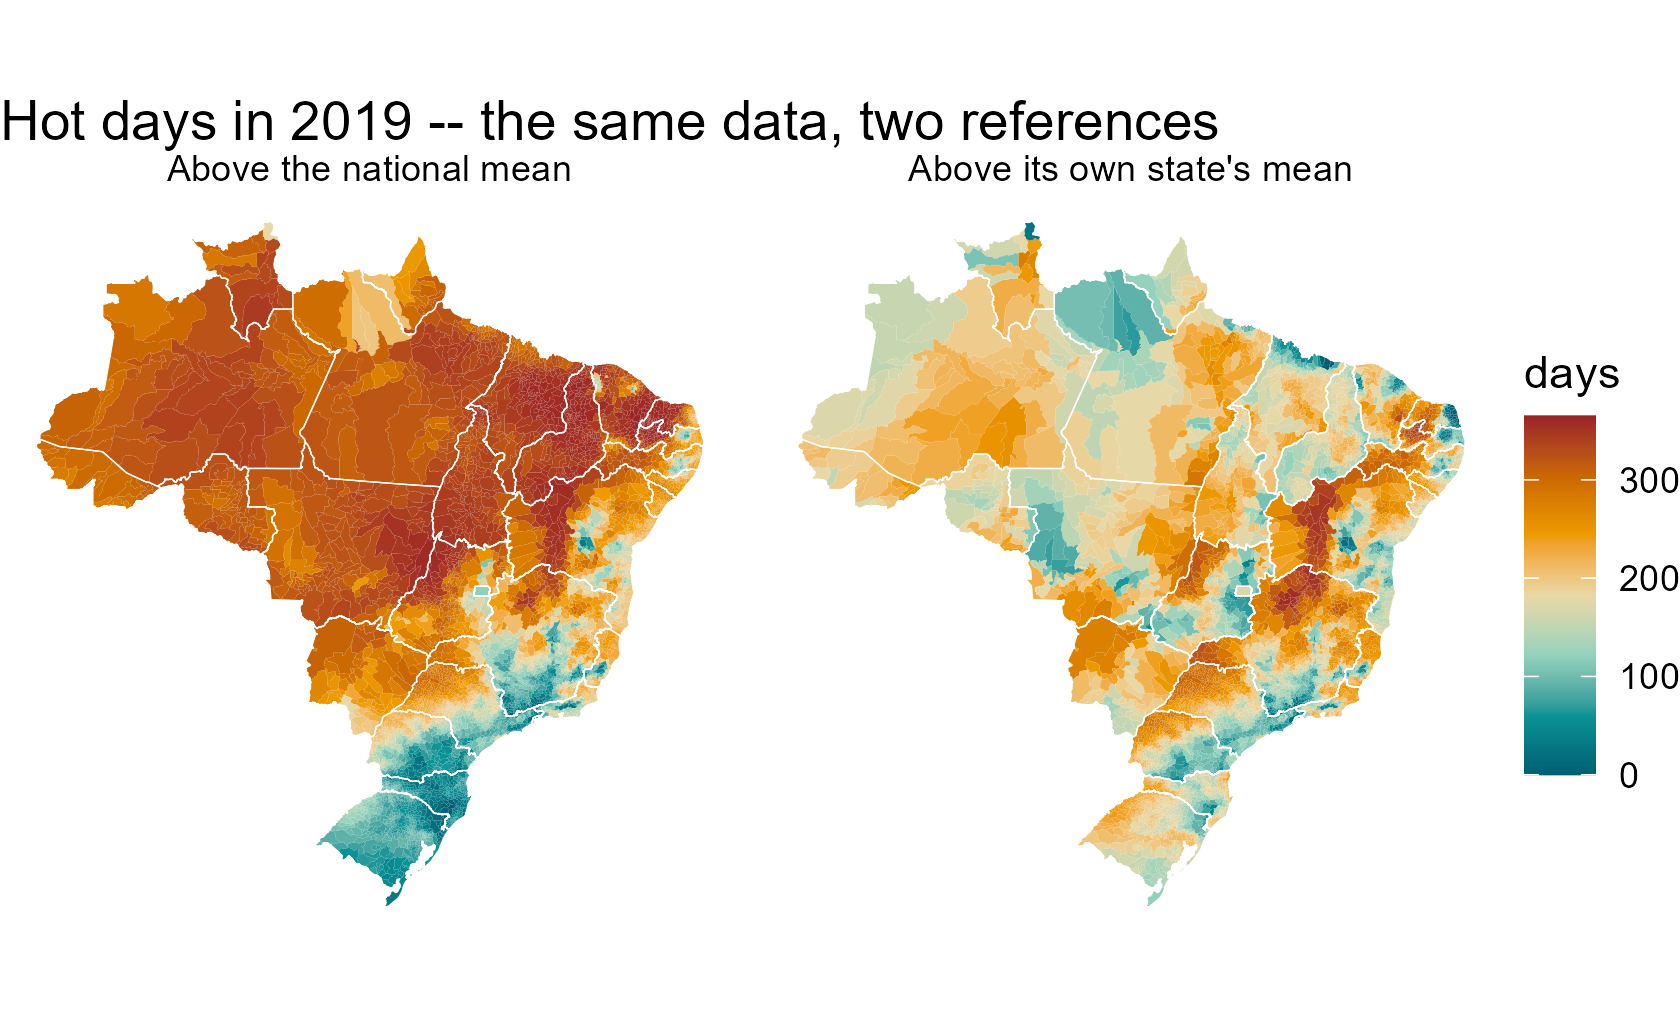
\includegraphics[width=\textwidth]{fig12_hot_reference}

      \vspace{2pt}
      \raggedright
      \scriptsize
      Same data, same year, same colour scale. What changes is \textbf{one
      \code{group\_by}} --- the mean is taken over the country, or over each
      state. On the left you are looking at Brazil's climate. On the right the
      state borders become visible, because every municipality is now being
      compared with the state it sits in.
    \end{column}
  \end{columns}
  \src{\code{climate\_data\_in\_R.R} § 3.2 and § 4}
\end{frame}

% --- PARKED: "The map", the single baseline choropleth that used to be this
% --- frame. The colour = NA point is worth keeping somewhere.
% \begin{frame}[fragile]{The map}
%   \begin{columns}[T]
%     \begin{column}{0.50\textwidth}
%       \vspace{-4pt}
% \begin{Rcode}
% ggplot(map_df) +
%   geom_sf(aes(fill = hot_days),
%           colour = NA) +
%   geom_sf(data = uf, fill = NA,
%           colour = "white",
%           linewidth = 0.15) +
%   scale_fill_gradientn(
%     colours = CLIM$seq) +
%   coord_sf(xlim = c(-74.1, -34.7),
%            ylim = c(-33.8,   5.4))
% \end{Rcode}
%       \vspace{-2pt}
%       \scriptsize
%       \textbf{\code{colour = NA}} is not cosmetic. $5{,}565$ outlines at slide
%       scale merge into a dark wash and hide the fill entirely. The state layer,
%       thin and on top, does the orientation instead.
%     \end{column}
%     \begin{column}{0.48\textwidth}
%       \centering
%       \includegraphics[width=\textwidth]{fig04_map_baseline}
%     \end{column}
%   \end{columns}
%   \src{\code{climate\_data\_in\_R.R} § 4.3 [SLIDE]; following Milz (2020)}
% \end{frame}

% ---------------------------------------------------------------------
% Section 5, the two comparisons. Both figures are ggplot objects the class
% script builds live (fig10 and fig11); the PNGs are the same objects saved.
\begin{frame}{Two cities, one year}
  \begin{columns}[T]
    \begin{column}{0.55\textwidth}
      \centering
      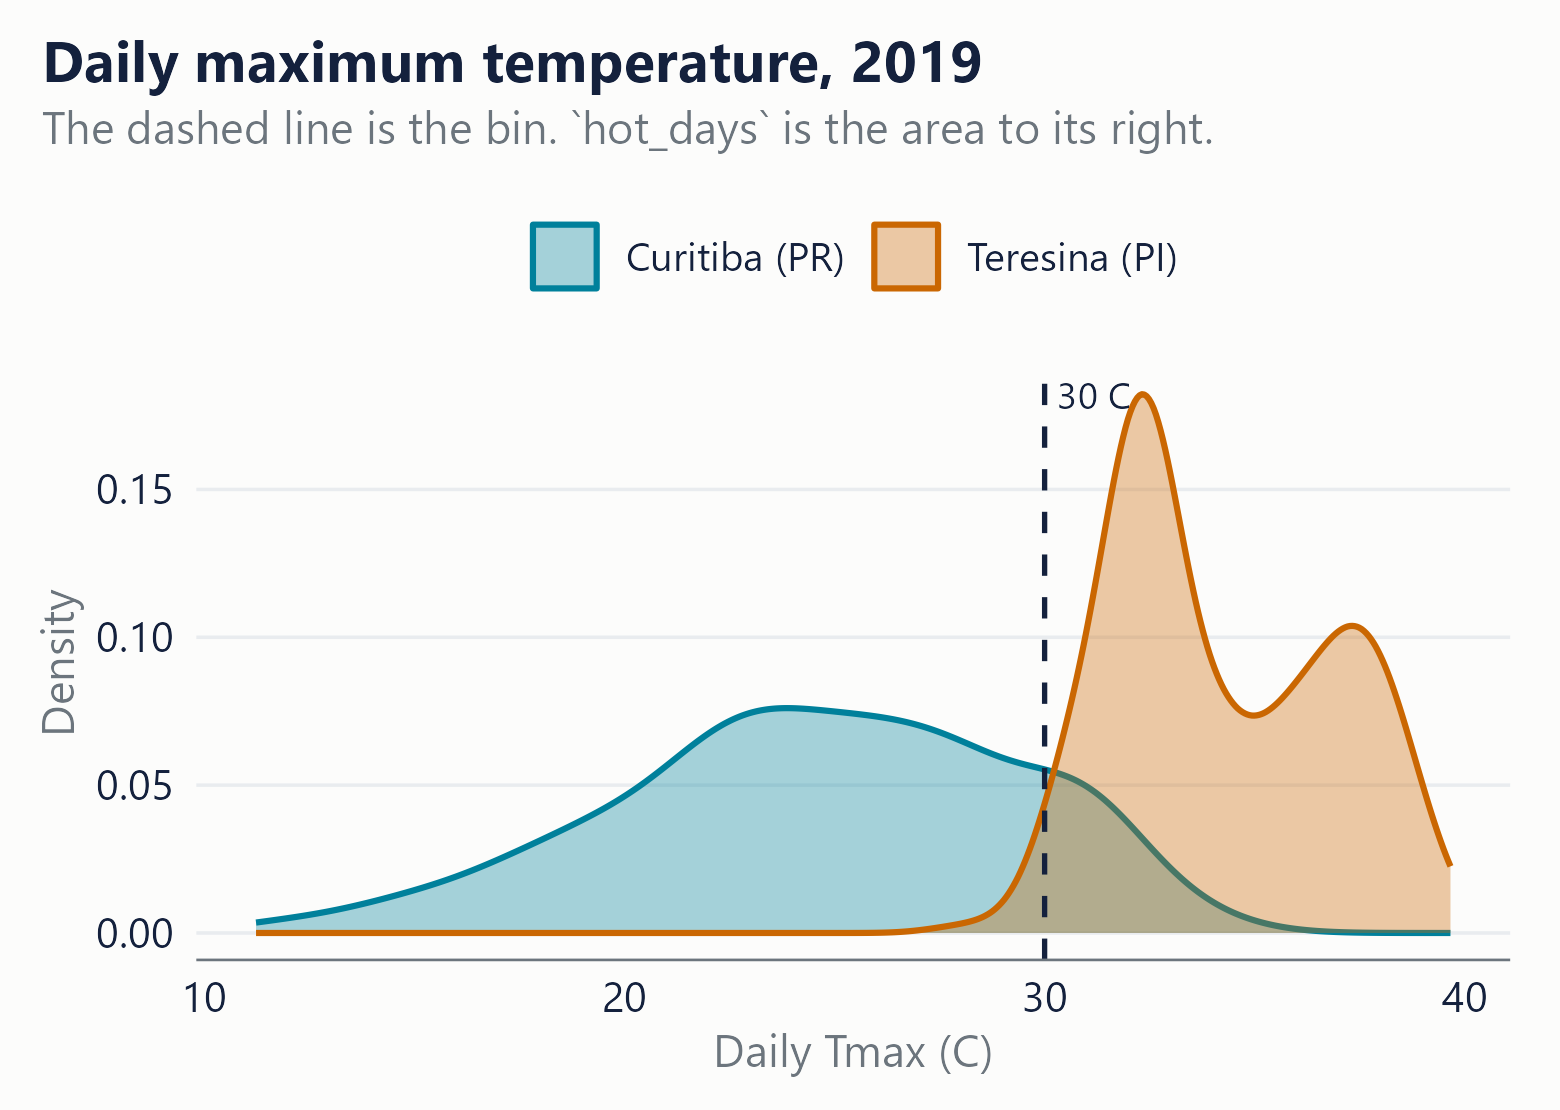
\includegraphics[width=0.90\textwidth]{fig10_two_cities}
    \end{column}
    \begin{column}{0.43\textwidth}
      \small
      The script does not pick these two. Of the five cities it follows, it takes
      the \emph{highest} and \emph{lowest} annual \code{tmean} in 2019 and asks
      who they are.
      \vspace{5pt}

      \centering
      \begin{dfbox}{lrrr}
        & mean $T_{\max}$ & sd & $\geq30$ \\
        \midrule
        Curitiba (PR) & 24.6 & 4.8 & 57 \\
        Teresina (PI) & 34.2 & 2.6 & 359 \\
      \end{dfbox}
    \end{column}
  \end{columns}
  \vspace{-1pt}
  \begin{itemize}
    \small\setlength{\itemsep}{1pt}
    \item \textbf{\code{hot\_days} is not a rival to the distribution --- it
          \emph{is} the distribution}, read once, at one place: the area right of
          the dashed line. Every threshold count in this class is this picture
          with the curve rubbed out.
    \item \textbf{The hotter city is the narrower one}, and the same count means
          different things in each: Curitiba's 57 hot days are its entire right
          tail, Teresina's 359 are its ordinary Tuesday.
  \end{itemize}
  \src{\code{climate\_data\_in\_R.R} § 5.1}
\end{frame}

% ---------------------------------------------------------------------
\begin{frame}{One city, two years}
  \begin{columns}[T]
    \begin{column}{0.55\textwidth}
      \centering
      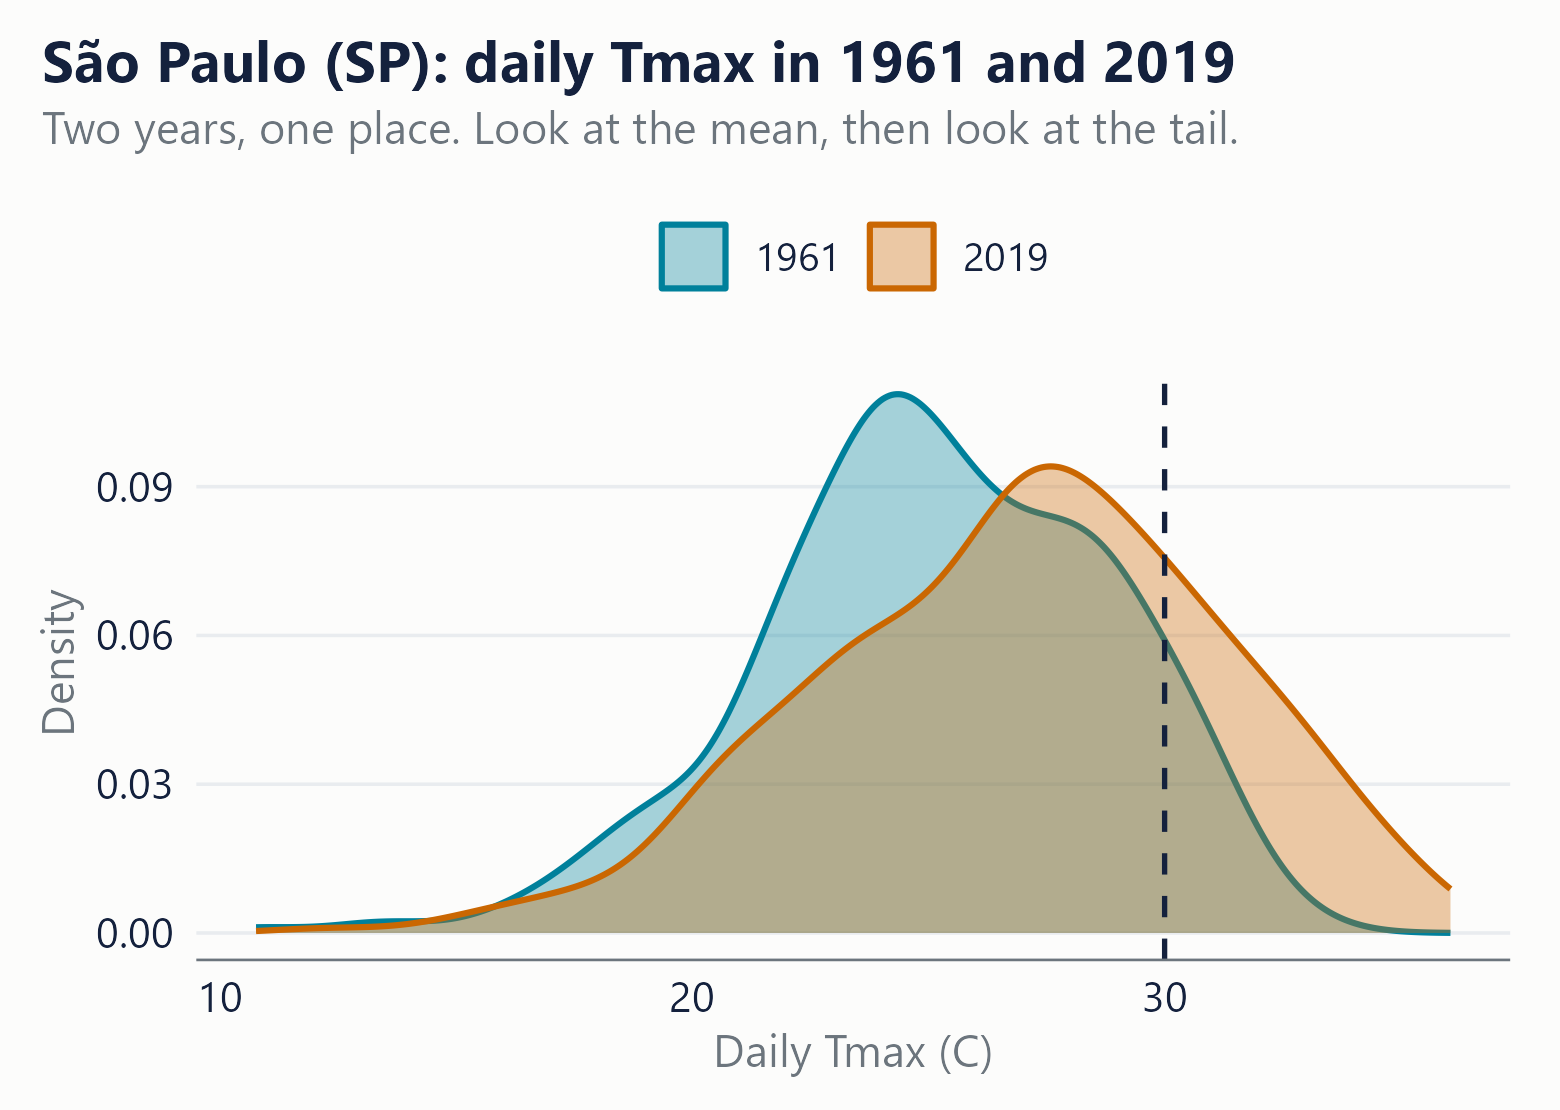
\includegraphics[width=0.86\textwidth]{fig11_two_years}
    \end{column}
    \begin{column}{0.43\textwidth}
      \small
      Same city, same calendar, fifty-eight years apart. \code{CITY\_ONE} is a
      knob --- put your own city in it and rerun.
      \vspace{5pt}

      \centering
      \begin{dfbox}{lrrrr}
        & mean $T_{\max}$ & sd & p90 & $\geq30$ \\
        \midrule
        1961 & 25.1 & 3.7 & 29.9 & 35 \\
        2019 & 27.0 & 4.3 & 32.5 & 92 \\
        \midrule
        $\Delta$ & \textcolor{climorange}{+1.8} & +0.6 &
          \textcolor{climorange}{+2.7} & $\times2.6$ \\
      \end{dfbox}
    \end{column}
  \end{columns}
  \vspace{-5pt}
  \begin{itemize}
    \small\setlength{\itemsep}{1pt}
    \item \textbf{The curve did not slide --- it slid \emph{and} widened.} The
          mean moves 1.8\,\textdegree C, the 90th percentile 2.7; days at or
          above 30\,\textdegree C go from 35 to 92. Report the mean and you have
          described the smaller half of what happened.
    \item And the count moved far more than the mean did: $+1.8$\,\textdegree C
          on the average, but $\times 2.6$ on the days above 30. \textbf{Which
          number you put in a regression is a claim about which part of the
          distribution does the damage.}
  \end{itemize}
  \src{\code{climate\_data\_in\_R.R} § 5.2}
\end{frame}

% =====================================================================
\partframe{Closing}{What to take away}
% =====================================================================

% ---------------------------------------------------------------------
\begin{frame}{Concluding remarks}
  \begin{enumerate}
    \small
    \item Brazilian climate data is easy to get and easy to misuse. The shortcut
          that saves you an afternoon has already chosen your product, your
          boundary year and your spatial weighting --- report all three, because
          \code{brclimr}'s own methodology page does not.
    \item You almost never need the file. The BR-DWGD parquet is \textbf{1.9\,GB}
          and $484{,}596{,}216$ rows; \code{arrow} and DuckDB read its footer over
          HTTP, touch only the blocks that could match, and hand back the two
          years we asked for in \textbf{2 seconds}. What ships to this class is
          $4{,}063{,}910$ rows in \textbf{20\,MB}.
    \item Read the source of small packages. \code{fetch\_data()} is a query
          against a public URL --- once you have seen it written out, you can
          write it yourself, against any parquet anywhere.
    \item \textbf{``A hot day'' is not a fact about the weather. It is a
          threshold you chose.} The same 2019 data, counted above the national
          mean and above each state's own mean, are two different maps, and one
          \code{group\_by} is the entire difference between them.
    \item Warming is not a shift. In São Paulo the mean $T_{\max}$ rose
          $1.8\,^\circ$C between 1961 and 2019 while days at or above
          $30\,^\circ$C went from 35 to 92. Report the mean and you have
          described the smaller half of what happened.
    \item \textbf{The join that works is the one to distrust.} Every polygon
          found a key, and nine municipalities are still empty --- Ilhabela among
          them, because the $0.1^\circ$ grid never covered the island.
          \code{ggplot} draws them in grey and says nothing.
  \end{enumerate}
\end{frame}

% ---------------------------------------------------------------------
% Two frames rather than one: the papers and the software the class actually
% ran on, then everything a student would go looking for afterwards. Every
% address here is a live \wl link, so the PDF is the handout.
\begin{frame}{References}
  \footnotesize
  \begin{itemize}
    \setlength{\itemsep}{2pt}
    \item Xavier, A. C., B. R. Scanlon, C. W. King \& A. I. Alves (2022). ``New
          improved Brazilian daily weather gridded data (1961--2020).''
          \emph{International Journal of Climatology} 42(16): 8390--8404.
          \dsub{The grid everything today runs on.}
    \item Schlenker, W. \& M. J. Roberts (2009). ``Nonlinear temperature effects
          indicate severe damages to U.S.\ crop yields under climate change.''
          \emph{PNAS} 106(37): 15594--15598. \dsub{Where the threshold count
          comes from.}
    \item \dsub{From Class 1:} Dell, Jones \& Olken (2014), \emph{JEL} 52(3):
          740--798. --- Jones, Moscona, Olken \& von Dessauer (2026), NBER WP
          34671.
  \end{itemize}
  \vspace{6pt}
  {\footnotesize\textbf{Packages}}\ \ {\footnotesize Saldanha, R. F.,
  \emph{brclimr} ---
  \wl[https://rfsaldanha.github.io/brclimr/articles/methodology.html]%
     {rfsaldanha.github.io/brclimr}, \emph{Articles \textgreater{}
  Methodology}. --- Pereira, R. H. M. \& C. N. Gonçalves, \emph{geobr} ---
  \wl{github.com/ipea/geobr}. Also \code{tidyverse}, \code{arrow},
  \code{duckdb}, \code{sf} and \code{glue}, all loaded through \code{pacman}.}
  \par\vspace{6pt}
  {\footnotesize\textbf{Learning R}}\ \ {\footnotesize Wickham, H. \& G.
  Grolemund, \emph{R for Data Science} --- \wl{r4ds.had.co.nz}; the
  \emph{tidyverse} itself --- \wl{tidyverse.org}.}
\end{frame}

% ---------------------------------------------------------------------
\begin{frame}{Where to go from here}
  \footnotesize
  \begin{itemize}
    \setlength{\itemsep}{4pt}
    \item \textbf{The exercise:} \wl{github.com/moraisnara/climate-course}
          --- one script, \code{exercise/climate\_data\_in\_R.R}, and the one
          CSV it reads. \dsub{The deck is in the same repository.}
    \item \textbf{Two tutorials in Portuguese, both by Beatriz Milz.}\\
          (2020) ``Criando mapas com os pacotes tidyverse e geobr'' ---
          \wl{beamilz.com/posts/2020-07-27-criando-mapas-com-os-pacotes-tidyverse-e-geobr}\\
          (2024) ``Dados espaciais com geobr'', Amostra R ---
          \wl{beatrizmilz.github.io/2024-09-amostra-geobr}
    \item \textbf{Shown today but not used.} INMET directly ---
          \wl{bdmep.inmet.gov.br} and
          \wl{portal.inmet.gov.br/dadoshistoricos}. The wrappers around it:
          \code{rmet}, \code{BrazilMet}, \code{climateBR}, \code{inmetpy}, and
          Base dos Dados (\code{br\_inmet\_bdmep}). Other products:
          TerraClimate, MODIS and INPE, ERA5 (ECMWF / Copernicus).
  \end{itemize}
  \vfill
  \centering{\color{climteal}\Large Questions?}
\end{frame}

\end{document}
